%% ===========================================================================
%% Communication Topology, Cross-Model Agreement, and the Limits of
%% LLM-Judged Verification in Automated Code Review.
%%
%% IEEE conference paper (IEEEtran). Overleaf: paste this file, Compiler =
%% pdfLaTeX. IEEEtran.cls ships with Overleaf. Insert the architecture-ladder
%% figure where marked in Section III-B (placeholder filename below).
%% All numeric results are from the pre-registered campaign; raw artifacts are
%% archived in S3 and replay deterministically with zero LLM calls.
%% ===========================================================================
\documentclass[conference]{IEEEtran}
\IEEEoverridecommandlockouts
\usepackage{cite}
\usepackage{amsmath,amssymb,amsfonts}
\usepackage{graphicx}
\usepackage{booktabs}
\usepackage{textcomp}
\usepackage{xcolor}
\usepackage{url}

\begin{document}

\title{Communication Topology, Cross-Model Agreement, and the Limits of\\
LLM-Judged Verification in Automated Code Review}

\author{\IEEEauthorblockN{En-Ping Su, Tong Wu, Shiting Huang, Mengshan Li}
\IEEEauthorblockA{\textit{Khoury College of Computer Sciences} \\
\textit{Northeastern University}, Vancouver, Canada}}

\maketitle

\begin{abstract}
Multi-agent frameworks are increasingly proposed for LLM-based code review, but
it is unclear whether the \emph{communication topology} among agents---rather
than the mere presence of multiple agents---improves review quality, or merely
adds cost. We run a pre-registered, controlled study that holds the model,
prompts, and specialist roles fixed and varies only the topology across a
four-rung ladder: a single-pass \textbf{Agentless} baseline, three uncoordinated
\textbf{Generalists}, a \textbf{Hierarchical} manager-plus-specialists
architecture, and a \textbf{Decentralized Consensus} architecture. We evaluate on
1{,}188 reviews over 99 PRs with injected defects (objective ground truth), 600
reviews over 50 PRs with human review comments, and 627 reviews over 30 PRs from
a live industrial portal with no ground truth. Three findings emerge. First,
\emph{homogeneous topology adds no capability}: the single-pass baseline is
F1-unbeatable, role specialization is statistically null ($p{=}0.74$), and
self-consistency filtering does not rescue the multi-agent arms; more agents buy
recall at up to $5\times$ the cost per true positive. Second, the measurable
value lies on a \emph{verification} axis: agreement between \emph{independent
model families} is a precision instrument---findings corroborated by all three
families are judged genuine at 89\% versus 54\% for same-model self-recurrence,
and the signal is judge-invariant ($\kappa{=}0.95$). Third, this instrument does
\emph{not} transfer to real, unlabeled industrial code: cross-family agreement is
rare and the LLM ``genuine-or-not'' judges disagree at $\kappa{=}0.03$, so the
precision-by-depth relationship is dominated by judge choice, not corroboration.
We conclude that multi-agent value in code review lies in cross-model
verification rather than communication topology, and that this verification
signal is bounded by the availability of a trustworthy correctness oracle.
\end{abstract}

\begin{IEEEkeywords}
Large Language Models, Multi-Agent Systems, Automated Code Review, Evaluation,
Ensembles, LLM-as-a-Judge.
\end{IEEEkeywords}

\section{Introduction}
Code review gates most software changes, and Large Language Models (LLMs) now
plausibly automate parts of it. A prominent design direction decomposes the task
among specialized agents that communicate---as in ChatDev~\cite{chatdev} and
MetaGPT~\cite{metagpt}. Yet most evaluations compare a \emph{whole} multi-agent
system against a single model, conflating two variables: how many agents there
are, and how they are organized and communicate. A centralized manager may be
cheaper; decentralized discussion may catch more cross-component issues; or the
extra structure may add cost without adding accuracy. We therefore ask:

\begin{quote}
\textbf{RQ:} Holding the model, prompts, and roles fixed, does the
\emph{communication topology} of a multi-agent system change the effectiveness
and efficiency of automated code review?
\end{quote}

We compare four architectures on a single ``ladder'' from no coordination to
full peer discussion (Fig.~\ref{fig:ladder}). Agentless is a strong single-LLM
baseline, since simple non-agent pipelines are competitive on software
tasks~\cite{agentless}. To isolate topology we reuse identical specialist
implementations and prompts across the multi-agent arms.

Because a benchmark result is only as trustworthy as its evaluation, we evaluate
on three complementary datasets---injected-defect ground truth, human-reviewer
agreement, and a live industrial repository---and we pre-register the hypotheses
and analysis. Our contributions are:
\begin{itemize}
  \item A controlled, pre-registered comparison in which communication topology
  is the only independent variable, over 2{,}415 reviews on three datasets.
  \item Evidence that \emph{homogeneous} multi-agent topology adds no capability:
  the single-pass baseline is F1-unbeatable and specialization is null.
  \item Identification of a \emph{cross-model verification} axis where multi-agent
  value actually lives---agreement between independent model families is a
  judge-invariant precision instrument.
  \item An external-validity boundary: on real unlabeled code the verification
  instrument fails, because LLM correctness judges become unreliable
  ($\kappa{=}0.03$)---a cautionary result for LLM-judged evaluation at large.
\end{itemize}

\section{Related Work}
\subsection{LLM-based software engineering and Agentless}
LLMs are applied to repair, localization, and review; SWE-bench established that
realistic GitHub tasks are hard for language models~\cite{swebench}. Agentless
questions whether autonomous agent systems are necessary, showing a simple
pipeline is competitive~\cite{agentless}. It is therefore the natural baseline
for asking whether multi-agent communication adds measurable value.

\subsection{Multi-agent software engineering}
ChatDev models development as communication among role agents~\cite{chatdev};
MetaGPT adds structured workflows to reduce inconsistency~\cite{metagpt}. Surveys
find the area promising but under-evaluated~\cite{survey}, and recent work
catalogs \emph{why} multi-agent LLM systems fail---coordination overhead,
cascading errors, weak verification~\cite{failures}. These failure modes are
properties of communication structure, motivating a controlled topology
comparison rather than a whole-system one.

\subsection{LLM-as-a-judge and ensembles}
Using a separate LLM to judge outputs scales evaluation~\cite{llmjudge}, but
judges exhibit biases including self-preference~\cite{selfpref}. We use LLM judges
in two distinct roles: an \emph{objective} same-issue matcher (does finding A
describe the same problem as finding B?) and a \emph{subjective} genuineness
judge (is this a real defect?). A central result of this paper is that the first
is reliable while the second is not, which bounds how far LLM-judged verification
can be trusted.

\section{Study Design}
\subsection{Independent variable: the four-rung ladder}
The independent variable is communication topology
(Fig.~\ref{fig:ladder}): (1)~\textbf{Agentless}---one LLM reviews the diff in a
single pass; (2)~\textbf{Generalists-3}---three general reviewers run
independently with no coordination (isolating ``more agents'' from ``more
structure''); (3)~\textbf{Hierarchical}---a manager assigns work to frontend,
backend, and database specialists and deterministically synthesizes their
findings; (4)~\textbf{Consensus}---the same specialists review independently, then
exchange findings and vote. Model (Claude Haiku 4.5), prompts, roles, and the
per-PR snapshot are held fixed; each (PR, arm) is the mean of 3 runs.

\begin{figure*}[t]
  \centering
  % === ARCHITECTURE FIGURE (placeholder) ===
  % fig1_architectures.png exists in docs/paper/ but shows only THREE panels
  % (Agentless / Hierarchical / Consensus). TODO before submission: extend it to
  % all FOUR ladder arms by adding the uncoordinated Generalists-3 rung, then
  % keep this filename (or swap in the updated asset).
  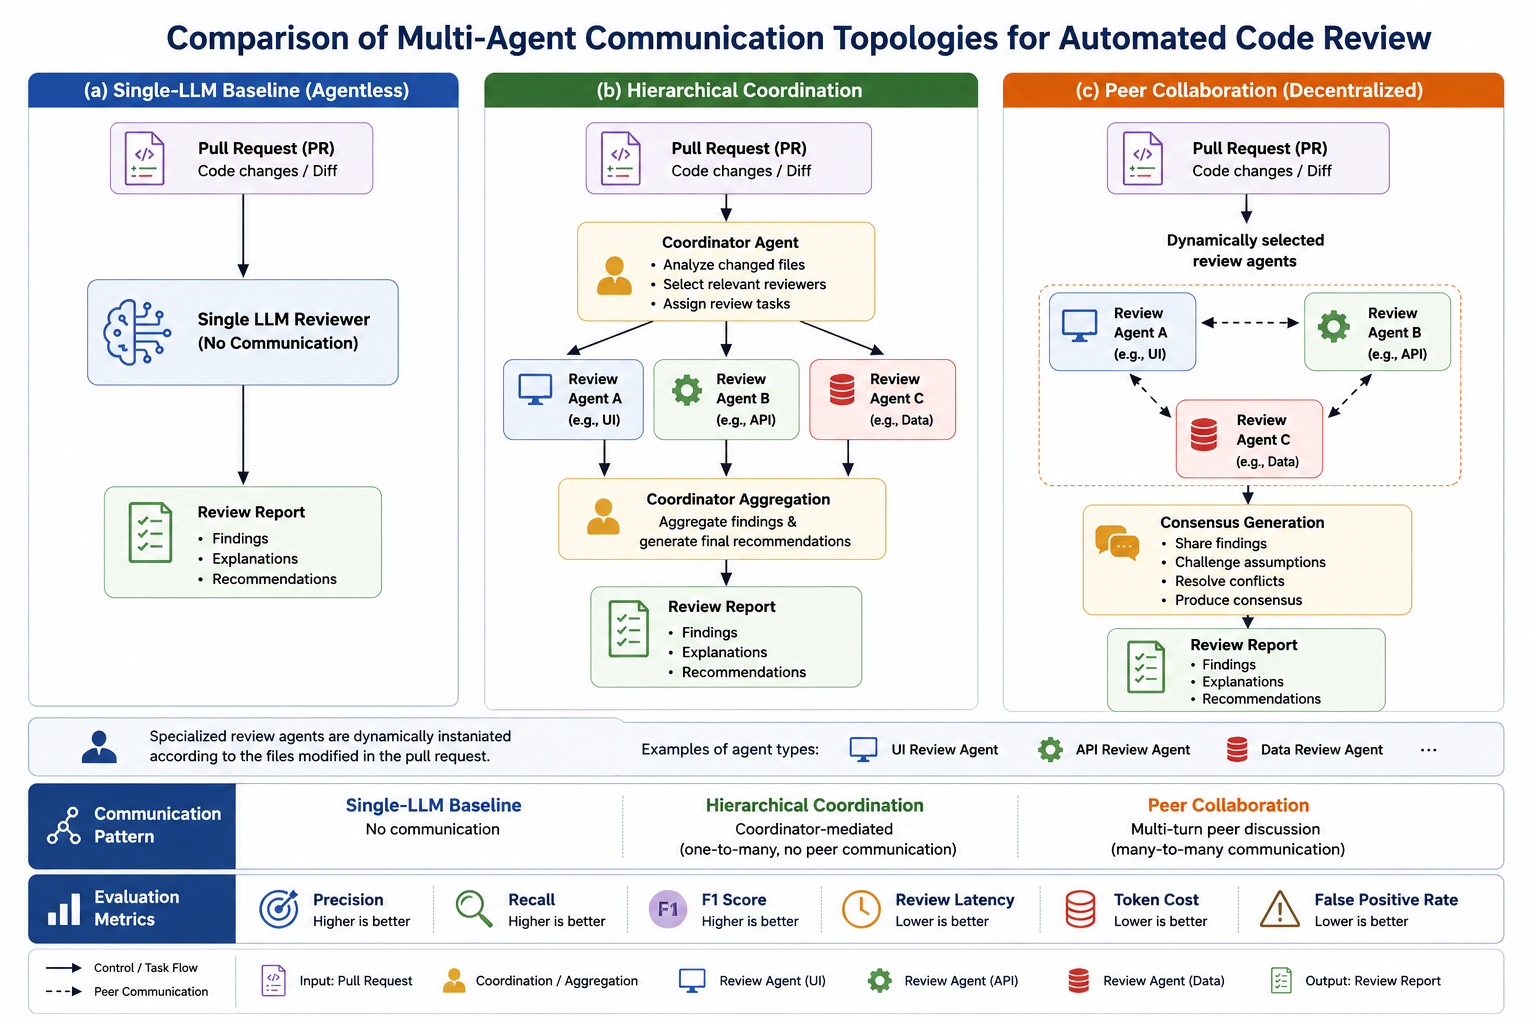
\includegraphics[width=\textwidth]{fig1_architectures.png}
  \caption{The four-rung communication-topology ladder. From left: \textbf{(a)}
  Agentless (single-pass, no communication); \textbf{(b)} Generalists-3 (three
  independent reviewers, no coordination); \textbf{(c)} Hierarchical (a
  coordinator assigns to specialists and aggregates---one-to-many, no peer
  communication); \textbf{(d)} Decentralized Consensus (specialists review, then
  discuss and vote---many-to-many). Solid arrows are control/task flow; dashed
  arrows are peer communication. \emph{[Placeholder---insert figure.]}}
  \label{fig:ladder}
\end{figure*}

\subsection{Datasets}
\textbf{E1 --- Qodo PR-Review-Bench}~\cite{qodo}: 99 PRs with injected defects and
explicit ground truth ($4\ \text{arms}\times3\ \text{runs}=1{,}188$ reviews).
Supports objective precision/recall/F1. \textbf{E2 --- SWE-PRBench}~\cite{sweprb}:
50 real PRs with human review comments (600 reviews); metrics measure agreement
with human reviewers. \textbf{E3 --- RAP Portal}: 30 real merged PRs from an
actively developed full-stack industrial portal (627 reviews); no authoritative
ground truth, so correctness is replaced by corroboration.

\subsection{Metrics and cross-family verification}
On E1 we report precision, recall, and F1 with a semantic matcher (an LLM decides
whether a produced finding matches a ground-truth defect, $\tau{=}0.7$). On E2 we
report coverage of human comments. On E3, lacking ground truth, we compute
\emph{corroboration depth}: independent findings are clustered by an LLM
pair-judge (Nova Pro, $\tau_{\text{pair}}{=}0.7$, union-find), and a cluster's
\emph{depth} is the number of independent \emph{model families} (Haiku, Kimi
K2.5, GLM 5) that produced it. We report the fraction of clusters a second LLM
judge rates \emph{genuine} at each depth---a proxy for precision. Across all
datasets we also collect operational cost: latency, tokens, LLM calls, and
inter-agent messages.

\subsection{Analysis and pre-registration}
Hypotheses and the analysis plan are pre-registered. PR is the unit; contrasts
use paired Wilcoxon signed-rank tests, Cliff's~$\delta$, seeded 2{,}000-iteration
bootstrap CIs, and Holm--Bonferroni correction within each hypothesis family.
Every raw review, judge verdict, and pair score is cached and archived, so all
statistics replay deterministically with zero further LLM calls.

\section{Results}
\subsection{Homogeneous topology adds no capability (E1)}
Table~\ref{tab:e1} gives per-arm means over 99 Qodo PRs. The single-pass baseline
has the \emph{best} F1 and by far the best precision; every multi-agent arm is
worse on F1 (paired semantic-F1 differences $+0.117$ to $+0.144$, all Holm
$p<0.001$, $\delta\ 0.30$--$0.36$). Crucially, the primary specialization
hypothesis is \textbf{null}: Hierarchical vs.\ Generalists-3 recall is
$0.624$ vs.\ $0.626$ (Wilcoxon $p{=}0.74$, $\delta{=}{-}0.005$) at comparable
precision---structuring the agents as specialists does not beat simply running
three of them. More agents buy \emph{recall} (Generalists-3 and Hierarchical
exceed Agentless on recall, Holm $p<0.001$), but at a large false-positive and
cost penalty: calls per confirmed true positive rise from $0.34$ (Agentless) to
$1.76$ (Consensus). On E2, coverage of human comments rises similarly
(Generalists-3 $0.68$ vs.\ Agentless $0.51$, Holm $p{=}0.001$) while F1 is a
four-way statistical tie. A pre-registered self-consistency filter (keep findings
recurring in $\geq k$ of 3 runs) does not bring any multi-agent arm within
$0.02$~F1 of the baseline.

\begin{table}[t]
\caption{E1 (Qodo, 99 PRs): per-arm means. Agentless is F1- and
precision-dominant; specialization (Hierarchical vs.\ Generalists-3) is null.}
\label{tab:e1}
\centering
\begin{tabular}{@{}lcccc@{}}
\toprule
\textbf{Arm} & \textbf{Precision} & \textbf{Recall} & \textbf{F1} & \textbf{Cost/TP} \\
\midrule
\textbf{Agentless} & \textbf{0.525} & 0.503 & \textbf{0.487} & \textbf{0.34} \\
Generalists-3 & 0.270 & \textbf{0.626} & 0.357 & 0.45 \\
Hierarchical  & 0.294 & 0.624 & 0.378 & 0.50 \\
Consensus     & 0.322 & 0.536 & 0.369 & 1.76 \\
\bottomrule
\end{tabular}
\end{table}

\subsection{The value is cross-model verification (E1)}
Value appears not \emph{within} a model's topology but \emph{across} independent
models. Table~\ref{tab:depth} (rows E1) shows the fraction of findings judged
genuine by corroboration depth. Same-model agreement (one model, three runs)
rises weakly with depth; \emph{cross-family} agreement (three model families)
rises sharply, reaching \textbf{89\%} genuine when all three families
independently produce a finding, versus \textbf{54\%} for same-model
self-recurrence. This depth signal is judge-invariant: re-scoring all candidate
pairs with an independent second pair-judge reproduces the table at
$\kappa{=}0.95$. In other words, agreement between \emph{different model families}
concentrates truth, whereas agreement between \emph{different topologies of the
same model} does not.

\begin{table}[t]
\caption{Corroboration-depth: fraction of clusters judged \emph{genuine} by the
number of independent sources agreeing. The cross-family precision gradient
(E1) does not replicate on real code (E3) under either genuine-judge.}
\label{tab:depth}
\centering
\begin{tabular}{@{}lccc@{}}
\toprule
\textbf{Sources agreeing} & \textbf{depth 1} & \textbf{depth 2} & \textbf{depth 3} \\
\midrule
E1 same-model ($\times3$ runs)      & 14\% & 17\% & 54\% \\
E1 cross-family (Haiku/Kimi/GLM)    & 28\% & 51\% & \textbf{89\%} \\
\midrule
E3 cross-family, judge = Nova Pro   & 100\% & 100\% & 100\% \\
E3 cross-family, judge = DeepSeek   & 15\% & 0\% & 0\% \\
\bottomrule
\end{tabular}
\end{table}

\subsection{The instrument does not transfer to real code (E3)}
On 30 real portal PRs the cross-family precision instrument fails---for two
independent reasons. First, \emph{agreement is rare}: only 23 findings reach
depth-2 and 5 reach depth-3 (of 904 clusters), versus 114 and 137 on E1; real,
diffuse review findings do not converge the way injected defects do. Second, and
more fundamentally, the \emph{genuineness judge is unreliable}. The two judges
disagree almost completely: Nova Pro rates 99\% of findings genuine (a rubber
stamp), DeepSeek 68\%, and their Cohen's $\kappa$ is $0.03$---barely above
chance. Consequently the depth$\rightarrow$precision relation is dominated by
judge choice (Table~\ref{tab:depth}, rows E3): under Nova it is flat at 100\%,
and under the discriminating judge it \emph{inverts}, with agreed-upon findings
scoring \emph{lower} (0\%) than solo findings (15\%). On real code, what
independent models converge on tends to be generic surface observations that a
strict judge rejects, not the injected defect all models catch on a benchmark.

What \emph{does} transfer is the operational structure (Table~\ref{tab:e3}). The
pool-coverage recall ladder is judge-independent and reproduces E1's ordering:
Agentless has the highest coverage ($0.27$) and Consensus the lowest ($0.10$)---
more agents again do not buy coverage. Precision, by contrast, is uninterpretable
because it swings entirely with the genuine-judge. Cost and communication scale
exactly as on the benchmarks: Consensus uses $9\times$ the LLM calls and
$13\times$ the latency of Agentless.

\begin{table}[t]
\caption{E3 (RAP Portal, 30 PRs). Recall (pool coverage) is judge-independent and
reproduces E1's ordering; precision swings with the judge; cost/communication
transfers cleanly.}
\label{tab:e3}
\centering
\small
\begin{tabular}{@{}lccccc@{}}
\toprule
\textbf{Arm} & \textbf{Recall} & \textbf{Prec.} & \textbf{Prec.} & \textbf{Calls} & \textbf{Latency} \\
 & (pool) & (Nova) & (DeepSeek) & & \\
\midrule
\textbf{Agentless} & \textbf{0.27} & 0.87 & 0.10 & 1 & 13\,s \\
Generalists-3 & 0.20 & 0.83 & 0.23 & 3 & 38\,s \\
Hierarchical  & 0.20 & 1.00 & 0.31 & 3 & 46\,s \\
Consensus     & 0.10 & 0.88 & 0.88 & 9 & 173\,s \\
\bottomrule
\end{tabular}
\end{table}

\section{Discussion}
Our results reframe where multi-agent value lies in code review. Communication
\emph{topology}---manager coordination, peer discussion---does not improve review
quality over a single pass; it improves recall at a steep cost, and specialization
is indistinguishable from uncoordinated generation. The measurable benefit of
using multiple models is \emph{verification}: independent model families agreeing
is a strong, judge-invariant precision signal on benchmark data. This suggests a
practical design---run a cheap single-pass reviewer across a few independent model
families and surface only cross-corroborated findings---rather than an elaborate
communication protocol over one model.

However, E3 exposes the precondition. The verification instrument depends on a
trustworthy correctness signal; on real, unlabeled code, LLM ``is-this-genuine''
judges disagree so severely ($\kappa{=}0.03$) that the instrument is not
measurable, even though the objective same-issue matcher remains reliable
($\kappa{=}0.95$). This is a cautionary result beyond code review: LLM-judged
\emph{correctness} is far less stable than LLM-judged \emph{equivalence}, and
pipelines that rely on the former on unlabeled data may be measuring their judge,
not their system.

\subsection{Threats to validity}
\emph{Construct:} E3 metrics are proxies and are labelled as such; no absolute
correctness is claimed there. \emph{Internal:} model, prompts, roles, and a
byte-identical per-PR snapshot are fixed across arms, so topology is the only
manipulated variable; the evaluation is deterministic and replays from cache.
\emph{External:} a single SUT model family and, on E3, a single industrial
repository (partly AI-authored) limit generalization; the three-dataset design
partly offsets this. \emph{Conclusion:} E3's depth-2/3 clusters are few (23/5),
so those CIs are wide; the reported non-replication is driven primarily by judge
unreliability, which is itself the finding.

\section{Conclusion}
Across 2{,}415 controlled reviews on three datasets, communication topology did
not improve automated code review: a single-pass baseline was F1-unbeatable,
specialization was null, and extra agents bought recall at up to $5\times$ the
cost per true positive. The value of multiple models lay instead on a
verification axis---cross-family agreement is a judge-invariant precision
instrument on benchmark data (89\% vs.\ 54\%). That instrument, however, did not
transfer to real unlabeled code, because LLM correctness judges became unreliable
($\kappa{=}0.03$). Multi-agent code review should therefore invest in cross-model
verification rather than communication topology---while recognizing that the
verification signal is only as trustworthy as the correctness oracle behind it.
Future work is a fixed-definition \emph{human} adjudication on real code, the one
oracle the LLM judges could not provide.

\begin{thebibliography}{00}
\bibitem{chatdev} C. Qian \emph{et al.}, ``ChatDev: Communicative agents for
software development,'' in \emph{Proc.\ ACL}, 2024.
\bibitem{metagpt} S. Hong \emph{et al.}, ``MetaGPT: Meta programming for a
multi-agent collaborative framework,'' in \emph{Proc.\ ICLR}, 2024.
\bibitem{agentless} C. S. Xia, Y. Deng, S. Dunn, and L. Zhang, ``Agentless:
Demystifying LLM-based software engineering agents,'' \emph{arXiv:2407.01489},
2024.
\bibitem{swebench} C. E. Jimenez \emph{et al.}, ``SWE-bench: Can language models
resolve real-world GitHub issues?'' in \emph{Proc.\ ICLR}, 2024.
\bibitem{survey} X. Zhang \emph{et al.}, ``LLM-based multi-agent systems for
software engineering: Literature review, vision and the road ahead,''
\emph{arXiv preprint}, 2024.
\bibitem{failures} Y. Li \emph{et al.}, ``Why do multi-agent LLM systems fail?''
\emph{arXiv preprint}, 2025.
\bibitem{llmjudge} L. Zheng \emph{et al.}, ``Judging LLM-as-a-judge with MT-Bench
and Chatbot Arena,'' in \emph{Proc.\ NeurIPS}, 2023.
\bibitem{selfpref} A. Panickssery \emph{et al.}, ``LLM evaluators recognize and
favor their own generations,'' \emph{arXiv:2404.13076}, 2024.
\bibitem{qodo} Qodo, ``PR-Review-Bench: a benchmark of pull requests with
injected review issues,'' code-review benchmark dataset, 2024.
\bibitem{sweprb} ``SWE-PRBench: pull-request review benchmark with human reviewer
comments,'' benchmark dataset derived from real GitHub PRs, 2024.
\end{thebibliography}

\end{document}
